% Chapter Template

\chapter{Implementation Details} % Main chapter title

\label{Chapter5} % Change X to a consecutive number; for referencing this chapter elsewhere, use \ref{ChapterX}

\lhead{Chapter 5. \emph{Implementation Details}} % Change X to a consecutive number; this is for the header on each page - perhaps a shortened title

%----------------------------------------------------------------------------------------
%	SECTION 1
%----------------------------------------------------------------------------------------

\section{Swan Application Layout}
In the process of implementing the support for SWAN WEAR and Beacon Based Sensor, SWAN application layout has changed dramatically.
We will cover the following main changes operated to SWAN project structure during the last 6 months:
\begin{itemize}
 \item Merging multiple SWAN repositories
 \item Splitting the SWAN project sources in libraries
 \item Uploading the SWAN JARS in publicly available repository - JCenter
\end{itemize}

Each of this changes had a big impact on SWAN and could bring unexpected bugs.


\subsection{Merging multiple SWAN repositories}
At the beginning of the master thesis project, the main repository of SWAN has holding the stable version of it, which was being used in production 
by a  company. Our SWAN project has a big team, each member work on different part of the SWAN or SWAN related functionality.
To avoid any breaking changes to the current SWAN version, I decided to make a different branch and put all my smartwatch related changes in it.
When I was done with implementing the first prototype of SWAN WEAR sensors, other PhD students' projects: SWAN Plus and IoT SWAN were also ready.
Unfortunately, the commits of the projects stated above were in different repositories so merging them into master branch was proven to be difficult.
We followed this procedure when merging the SWAN:
\begin{itemize}
 \item Create the release branch with the old, stable SWAN
 \item Create development branches for SWAN Plus and IoT SWAN
 \item Export commits from SWAN Plus and IoT SWAN as patches
 \item Apply the patches to each development branch
 \item Merge Smartwatch code into Master
 \item Merge SWAN Plus into master and resolve conflicts
 \item Merge IoT SWAN into master and resolve conflicts
\end{itemize}

The most challenging part was to apply patches from the two different repositories. Merging commits were the reason why some history was 
lost, and patches were hard to apply. This also proves why you should always use the rebase option instead of merging option when you push commits
to the remote. Atlassian article\cite{atlassian_merge_rebase} explains the main advantage of rebasing over using merging commits.

\subsection{Splitting SWAN sources into libraries}\label{scc:swan_split}
After the implementation of the smartwatch sensors and beacon sensors, as part of research topic, SWAN had to be ported on smartwatch.
There were multiple options of how I was supposed to handle the challenge:
\begin{itemize}
 \item Clone all SWAN code and adapt it for the smartwatch
 \item Extract all common code and make it a library
\end{itemize}

I choose the second option, since it will avoid duplicate code and will allow easier maintenance in the future. As a starting point, I decided to see if The Evaluation Engine
code can be extracted and called from a library. The dependencies were extensive. The Evaluation Engine was depending on:
\begin{itemize}
 \item Swan Interface code - Classes that applications need to communicate with SWAN
 \item Swan Song Implementation - Parser and Data structure implementation for SWAN Expression
 \item Sensor Interfaces - used to implement new sensors in SWAN
 \item Beacon Implementation
 \item Proximity Implementation (SWAN Plus)
\end{itemize}

The first three components were separated from the SWAN Phone application and added to the swan core. Unfortunately, the dependency on the last two items
was still present and it had to be removed from the code, since the implementation was relevant only for phone and not for the smartwatch.
To preserve the functionality, all the methods depending on Proximity Manager and Beacon Discovery were replaced with empty bodies and the Evaluation Engine on
the phone was sub-classing the Evaluation Engine in the library and implementing the missing functionality.
The same design was applied to Abstract SWAN Sensor who was relying on Sense Android Library to offload values[cite].

After \textbf{Swan Core} was made independent, we decided to extract \textbf{Swan Song} and \textbf{Swan Interface} from it and make them separate libraries.
The main reason for this library separation was the way applications interact with SWAN. Swan Interface are often imported as a separate jar in any application that want to register a 
SWAN expression. To improve the distribution of the Swan Interface, we decided to make it available on Android Main Repository - JCenter\cite{jcenter}. Uploading the Jars required us to follow the tutorial by The Cheese Factory\cite{jcenter_tutorial}.

Because we are maintaining the packages on JCenter now, the old packages and package building scripts  in the repository were discarded.
The JCenter  is not storing the packages in JAR format, but in the new format made to accommodate the Android Resources: AAR \cite{aar_format}. 
The new package format can be built and uploaded directly from Android Studio. Also, when changes are being operated on Swan Interface, 
the library versions should be updated accordingly:

\begin{itemize}
 \item If any change or addition  in the library was made, increment the patch version number: 1.0.0 $\rightarrow$1.0.1
 \item If any public class or Enumeration was deleted, increment the minor version: 1.0.0 $\rightarrow$ 1.1.0 
 \item The major version should be only incremented with SWAN major version: 1.0.0 $\rightarrow$ 2.0.0
\end{itemize}

More information about how to manage and upload swan libraries is available on SWAN wiki on Github\cite{swanWiki}

\section{Beacon based Bluetooth Sensors}

Bluetooth sensors allow us to get proximity data from the nearby beacons. Beacon sensor integration into SWAN expression based approach was not seamless.
The new data specifications which include beacon extension are discussed in \hyperref[Chapter3]{Chapter 3}.

Before exploring the implementation details we must discuss the available Beacon technology and Beacon Frame format.
The Bluetooth Low Energy Beacons can broadcast various data with different transmission power and broadcast interval.
The broadcast power is measured in dBm\cite{dbiRef}. The transmission power can vary from -30dBm and +4dBm. Higher transmit power
increase the range, but also shorten the battery life. The broadcast interval can vary from 300ms to more than 5 seconds. Higher resolution improves the accuracy of data,
especially for real-time applications, but also shorten the battery life.

To avoid the fragmentation of the Beacon Market, Google and Apple stepped in and proposed two standards for Beacon Frame Layout:
\begin{itemize}
 \item Apple iBeacon - simple beacon format, mostly used for proximity(distance measuring) applications
 \item Google Eddystone - complex standard, with 3 available frame formats:
 \begin{itemize}
  \item Eddystone UID - similar to iBeacon, broadcast unique ID
  \item EddystoneTLM - telemetry frame format, stores information about the beacon, such as temperature, battery level, number of packets sent
  \item Eddystone URL - frame layout which encodes a 17 bytes long URL in the frame
 \end{itemize}
\end{itemize}

The standards from above are industry recognized and widely implemented by various Beacon Manufacturers.
Unfortunately, even the Google Eddystone Format is not flexible enough and some companies need to come up with their own format to support extra functionality 
added to  their beacon products. We will also discuss the following frame formats which are proprietary to companies selling the test beacons, but they enable us to explore the
new way of using beacons:
\begin{itemize}
 \item AltBeacon Beacon Format - default beacon format present in the library used by SWAN for beacon scanning
 \item Estimote Nearable - Beacon Frame Format developed by Estimote\cite{estimote_company}, with accelerometer and movement data embedded into the format
\end{itemize}

The beacon implementation is revolving around adding support for the four beacon formats listed above. Implementation details were further split into 
following steps:
\begin{itemize}
 \item Implement Bluetooth Low Energy Scan
 \item Add support for existing Beacon Formats
 \item Implement Bluetooth Beacon Discovery
 \item Implement Bluetooth Based Sensors
\end{itemize}

\subsection{AltBeacon Library}
The AltBeacon Library is developed by Radius Networks company and provide a free and open-source implementation for applications that want to scan for beacons.
We choose to use this library over a custom implementation because of the easy way to add new beacon format. The library does not support beacons with encrypted 
identifiers, but it allows us to parse almost any existing, non-encrypting beacon frame. A proof of flexibility is our beacon layout for Estimote Nearable that we were able to 
implement in SWAN.
AltBeacon runs as a service, so SWAN needs to register to get the results of every scan. All the data from available beacons are available at once, so we decided to go for observer 
pattern, and register all sensors that want to access beacon data in our singleton class. This allows us to scan once for all sensors.

\subsection{Beacon Frame Formats}
The support for Apple iBeacon, Eddystone UID, Eddystone TLM, Eddystone URL and AltBeacon Format was already available in the library.
The Estimote format was left for us to analyse and provide the proper parsing expression to the AltBeacon Library.

The process of parsing the non- standard frame starts with finding the specifications for each byte in the frame. Fortunately, we found a NodeJs implementation 
who parses the Estimote Nearable Frame. The data encoded is presented in \hyperref[fig:estimote_format]{Figure 5.1}.
Before decoding the data we must tell the AltBeacon Library where to look for the frame identifier. The debugging mode allows us to see how the Bluetooth Low Energy frames are being parsed.

\subsection{Retrieving data from specific Beacons}
Original SWAN only allowed to return a single value of the primitive type. To comply with the new SWAN Data Specifications, we test the location part of expression to see which information we should provide:

\begin{itemize}
 \item If location is \textbf{self} we retrieve a random beacon from the list, which matches our frame type and give the result to the user
 \item if location contains a \textbf{beacon ID} we search for the beacon in list and if it is present, we will output the result
\end{itemize}

Other types of operations can be implemented, but first, a new revision of data formats should be made, to set the guidelines for all sensor implementations.

Our implementation relies on a singleton class which gets the result of the scanning and then distributes it to all registered beacon sensors. The AltBeacon library will automatically stop scanning
if no beacon sensors are registered.

\begin{figure}[htbp]
  \centering
    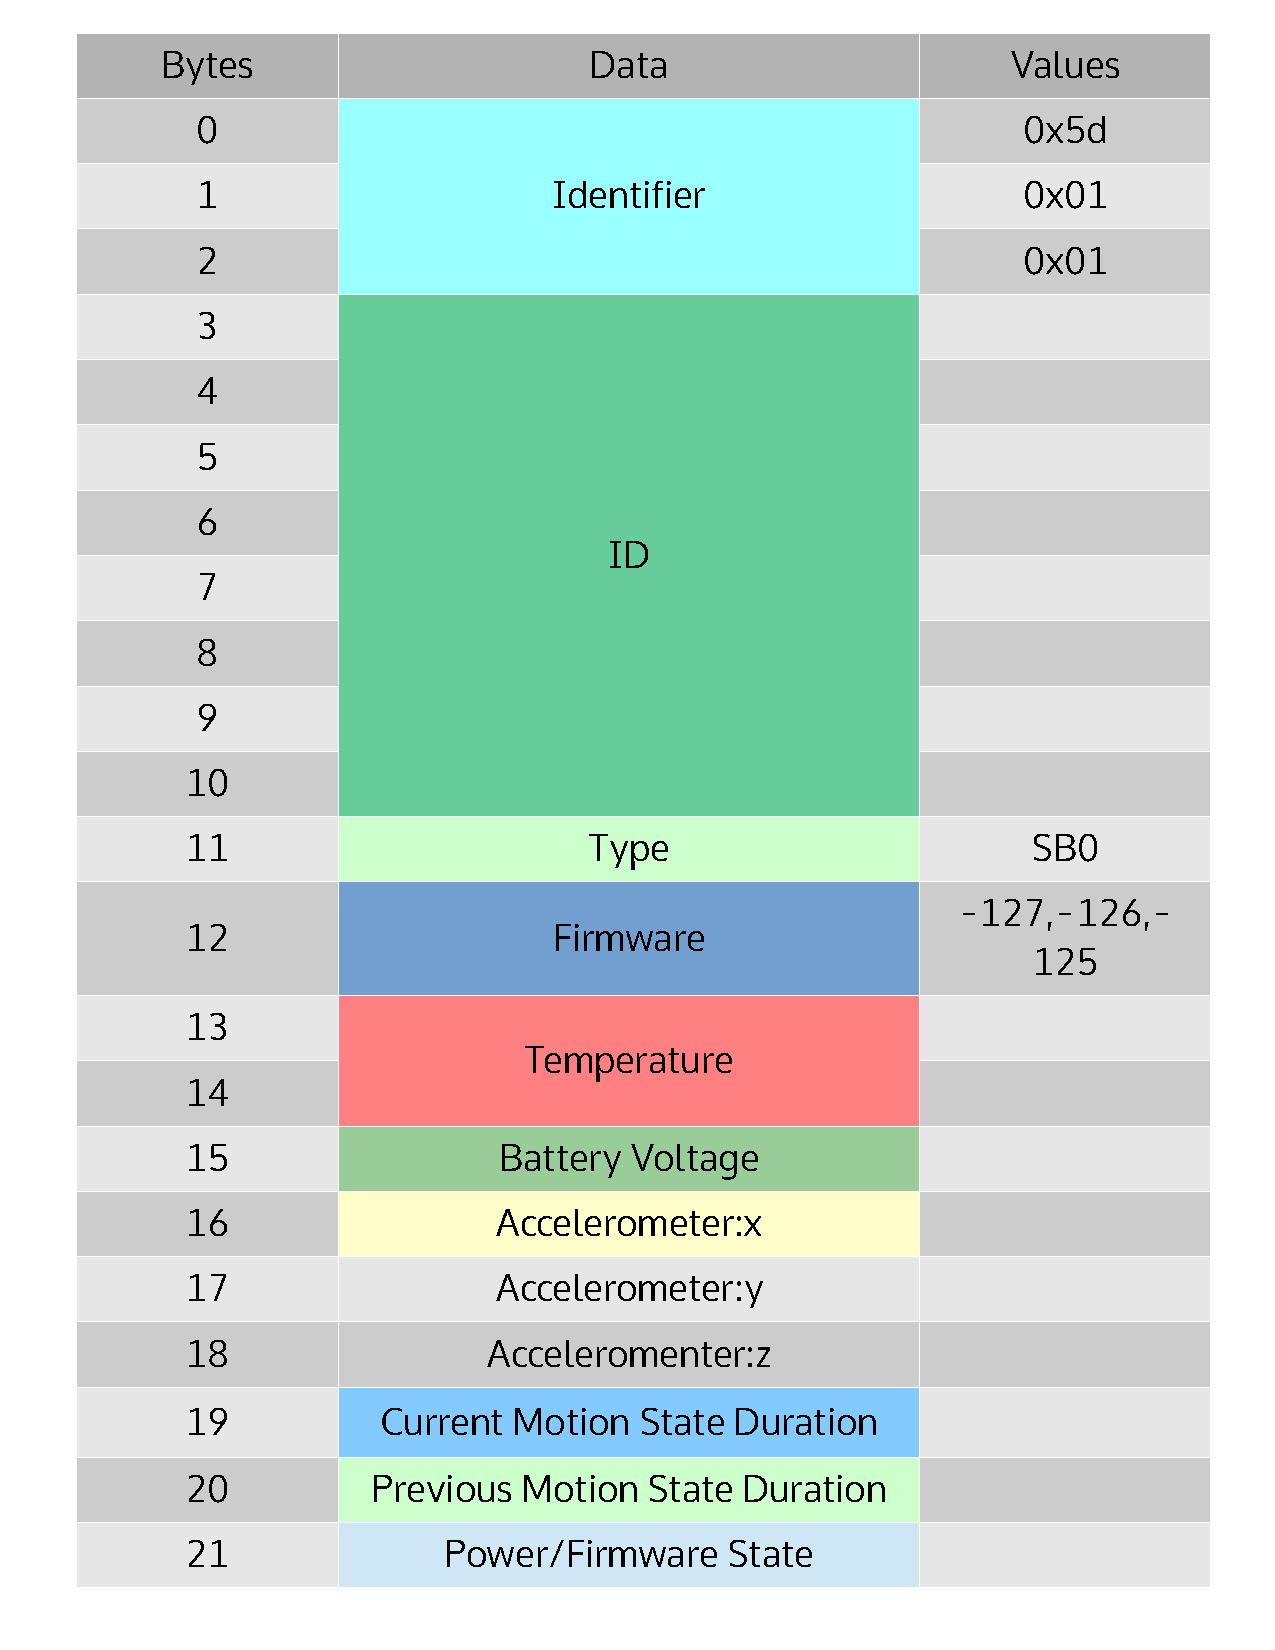
\includegraphics[scale=0.4]{Figures/data_format.pdf}
    \rule{35em}{0.5pt}
  \caption[Estimote Nearable Format]{Estimote Nearable Format}
  \label{fig:estimote_format}
\end{figure}

\section{ Value Based Smartwatch Sensors }
Implementing the value based smartwatch sensor was the first option and it derived from the Android's guidelines of performing the minimum amount of computation on the watch.
The other requirement was to keep code for Android Wear as small as possible, since the performance of the integrated components is lower compared to computing power on the smartphone.

To keep the implementation simple, we have a singleton class  responsible for communication between the smartphone and watch. We also issue start and stop commands to our service on the smartwatch,
so when no smartwatch sensor is active, the SWAN will not run on the watch.

We used the data path \cite{android_wear_datapath} for reliable communication between devices. The use of data path guarantee that the value will always be delivered at the cost of increased delay
and jitter\cite{jitter_ref} which affect our delay enforcing policy in SWAN.

The watch service is implemented as a foreground service\cite{foreground_service}. Running in foreground requires us to display the notification on the watch, but on the other hand we have the 
guarantee that our service will not be put to sleep by the operating system. 
Each SWAN sensor on the phone  is able to send start and stop commands, and the watch service will always count how many sensors are active. When no sensors are active, the service will stop.

Despite the Google's guidelines of keeping the Android Wear applications small, value based smartwatch sensors have poor energy efficiency. More about the power consumption experiment, 
in \hyperref[Chapter6]{Chapter 6}.

\section{Expression  Based  Smartwatch Sensors }

Expression based smartwatch sensor implementation aims to bring SWAN on your smartwatch. Before, we didn't consider to have SWAN on the watch a good idea. SWAN is a big application and running
it on the watch could result in sever performance issues on the watch. The opportunity on running SWAN on watch arisen after we managed to split SWAN source-code into \hyperref[scc:swan_split]{multiple libraries}. Some performance incurring features, such as database storage were left behind, and now the source-code was small enough to run on watch.

Compared to normal SWAN expression, a wear expression has the \hyperref[fig:SwanExpression]{location string} set to \textbf{wear} keyword. Evaluation Engine is responsible for changing the location
to \textbf{self} and forwarding the expression to SWAN on smartwatch.
The implementation of expression based smartwatch sensors added on top of the existing value based implementation. New commands were added to start and stop a swan expression on the watch.
The values sent back use the same implementation as for value based sensors. 

The main difference between value based and expression based sensors is that the values are not sent to SWAN sensor implementation for evaluation, but rather added to Evaluation Engine list of cached
values. This approach offers very low power consumption on the phone, as we can see from the power analysis in \hyperref[Chapter6]{Chapter 6}.
